\chapter{Application Pratique : Analyse de Risque LiZbiZ}
\label{chap:apprisque}

Ce chapitre met en œuvre la méthode EBIOS RM sur le cas concret de l'entreprise LiZbiZ. Nous suivrons les étapes méthodologiques pour aboutir à une estimation des risques.

\section{Étape 1 : Établissement du Contexte (Atelier 1)}

Avant de chercher les risques, il faut définir le cadre de l'étude.

\subsection{Définition du Périmètre}

\begin{boxlizbiz}
\textbf{Commande client :} La DSI de LiZbiZ demande une analyse de risques sur le périmètre \textbf{"Système d'Information Logistique"}.
Celui-ci englobe l'ERP (Odoo), la Base de Données Clients, et les terminaux de scan (IoT) dans l'entrepôt.
\end{boxlizbiz}

\subsection{Identification des Actifs Essentiels}

En EBIOS RM, on distingue les actifs \textbf{essentiels} (ce qui a de la valeur pour le métier) des actifs \textbf{supports} (la technique).

\begin{table}[htbp]
\centering
\begin{tabular}{p{4cm}p{7cm}}
    \toprule
    \textbf{Actif Essentiel} & \textbf{Description} \\
    \midrule
    Processus "Commande-Livraison" & Flux complet depuis la commande web jusqu'à l'expédition. Sensibilité : Critique (Arrêt = Perte de CA). \\
    Information "Données Clients" & Coordonnées, historique commandes, moyens de paiement. Sensibilité : RGPD. \\
    \bottomrule
\end{tabular}
\caption{Actifs Essentiels LiZbiZ}
\end{table}

\subsection{Identification des Actifs Supports}

Ce sont les éléments techniques qui portent les actifs essentiels (ceux du lab GNS3).

\begin{itemize}
    \item Serveur Web (DMZ) : Héberge le portail de commande.
    \item Serveur ERP (VLAN 20) : Héberge le processus métier.
    \item Base de Données PostgreSQL : Stocke l'information client.
    \item Réseau WiFi (VLAN 40) : Support des scanners logistiques.
\end{itemize}

% ------------------------------------------------------------------------------
\section{Étape 2 : Étude des Événements Redoutés (Atelier 2)}
% ------------------------------------------------------------------------------

\subsection{Définition}

\begin{boxdef}
\textbf{Événement Redouté :} Un incident potentiel, décrit du point de vue de l'impact métier. Il répond à la question : "De quoi a-t-on peur ?". Il se caractérise par une atteinte à un actif essentiel sur un critère (D, I, C, T).
\end{boxdef}

\subsection{Exemple pour LiZbiZ}

Nous identifions 2 événements redoutés majeurs pour l'actif "Données Clients" :

\begin{enumerate}
    \item \textbf{ER1 - Divulgation de données clients :}
    \begin{itemize}
        \item \textit{Critère :} Confidentialité (C).
        \item \textit{Impact :} Atteinte à la réputation, amende CNIL, perte de confiance clients.
        \item \textit{Gravité estimée :} 4 (Critique).
    \end{itemize}
    
    \item \textbf{ER2 - Indisponibilité du SI Logistique :}
    \begin{itemize}
        \item \textit{Critère :} Disponibilité (D).
        \item \textit{Impact :} Arrêt des expéditions, non-respect de la promesse "24h".
        \item \textit{Gravité estimée :} 5 (Catastrophique).
    \end{itemize}
\end{enumerate}

% ------------------------------------------------------------------------------
\section{Étape 3 : Analyse des Risques - Scénarios (Atelier 3)}
% ------------------------------------------------------------------------------

\subsection{Construction d'un Scénario de Menace}

Un scénario décrit \textbf{comment} une menace exploite une vulnérabilité pour provoquer l'événement redouté.

\begin{boxlizbiz}
\textbf{Scénario S1 : "Ransomware sur l'ERP"}
\begin{itemize}
    \item \textbf{Source de Menace :} Cybercriminels organisés (Motivation : Financière).
    \item \textbf{Menace :} Déploiement d'un Ransomware (Chiffrement malveillant).
    \item \textbf{Vulnérabilité exploitée :} 
    \begin{itemize}
        \item Serveur Web non mis à jour (Faille CVE).
        \item Absence de segmentation entre VLAN 10 et VLAN 20.
    \end{itemize}
    \item \textbf{Chemin d'attaque :} Le hacker compromet le serveur Web (DMZ) $\rightarrow$ Pivot vers le VLAN Applicatif $\rightarrow$ Chiffrement de l'ERP.
\end{itemize}
\end{boxlizbiz}

\subsection{Vraisemblance du Scénario}

La \textbf{Vraisemblance} est la probabilité que le scénario se réalise, compte tenu des défenses existantes.

\begin{table}[htbp]
\centering
\begin{tabular}{p{5cm}p{2cm}}
    \toprule
    \textbf{Défense existante chez LiZbiZ} & \textbf{Efficacité} \\
    \midrule
    Pare-feu pFsense (Filtrage) & Moyenne \\
    Antivirus sur serveurs & Faible (bases non à jour) \\
    Sauvegardes (Nightly) & Moyenne \\
    \textbf{Vraisemblance globale} & \textbf{Élevée (4)} \\
    \bottomrule
\end{tabular}
\caption{Estimation de la vraisemblance}
\end{table}

Le risque est d'autant plus plausible que les vulnérabilités sont connues et les défenses faibles.

% ------------------------------------------------------------------------------
\section{Étape 4 : Estimation et Hiérarchisation (Atelier 4)}
% ------------------------------------------------------------------------------

\subsection{Calcul de la Criticité}

Nous croisons la Gravité de l'Événement Redouté (ER2) avec la Vraisemblance du Scénario (S1).

\begin{itemize}
    \item \textbf{Gravité (Impact Business) :} 5 (Catastrophique - Arrêt total).
    \item \textbf{Vraisemblance (Facilité technique) :} 4 (Élevée - Failles connues).
\end{itemize}

\begin{center}
\textbf{Criticité du Risque = 5 x 4 = 20 / 25 (Risque Critique)}
\end{center}

\subsection{Cartographie des Risques (Heatmap)}

On positionne ce risque sur la matrice de visualisation pour le COMEX.

\begin{figure}[htbp]
\centering
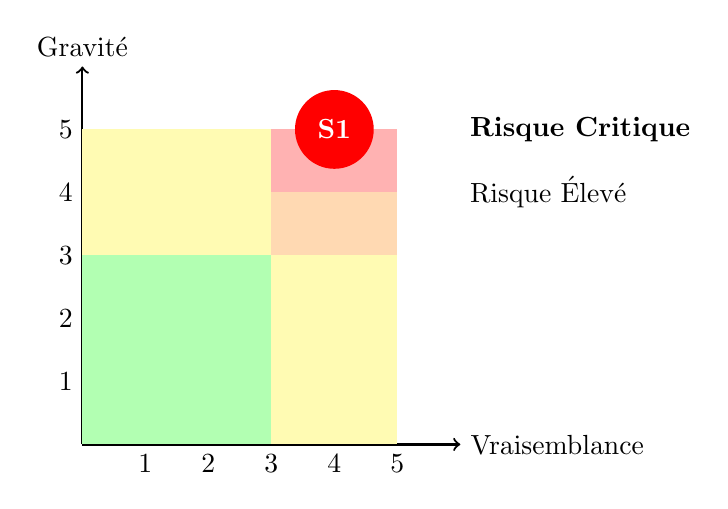
\begin{tikzpicture}[scale=0.8]
    % Axes
    \draw[thick,->] (0,0) -- (6,0) node[right] {Vraisemblance};
    \draw[thick,->] (0,0) -- (0,6) node[above] {Gravité};
    
    % Labels Axes
    \foreach \x in {1,...,5} {
        \node at (\x,0) [below] {\x};
        \node at (0,\x) [left] {\x};
    }
    
    % Zones de couleur
    \fill[green!30] (0,0) rectangle (3,3); % Faible
    \fill[yellow!30] (3,0) rectangle (5,3); % Moyen
    \fill[yellow!30] (0,3) rectangle (3,5); % Moyen
    \fill[orange!30] (3,3) rectangle (5,4); % Elevé
    \fill[orange!30] (4,3) rectangle (5,5); % Elevé
    \fill[red!30] (3,4) rectangle (5,5); % Critique
    
    % Le risque LiZbiZ
    \node[circle, fill=red, text=white, minimum size=1cm] at (4,5) {\textbf{S1}};
    
    % Légende
    \node[right] at (6,5) {\textbf{Risque Critique}};
    \node[right] at (6,4) {Risque Élevé};
\end{tikzpicture}
\caption{Positionnement du risque Ransomware chez LiZbiZ}
\end{figure}

% ------------------------------------------------------------------------------
\section{Travaux Pratiques : Première Mission}
% ------------------------------------------------------------------------------

\begin{boxlizbiz}
\textbf{Mission pour les étudiants :}

En utilisant le laboratoire GNS3 et les éléments fournis :
\begin{enumerate}
    \item Complétez la fiche de risque EBIOS pour le scénario S1.
    \item Identifiez un second scénario de risque concernant le \textbf{WiFi Logistique} (Indice : quel actif est sensible ? Quelle menace ?).
    \item Proposez une première mesure de réduction simple pour faire baisser la vraisemblance du scénario Ransomware.
\end{enumerate}
\end{boxlizbiz}

% ==============================================================================
% Fichier : 02_module_risque.tex (Extrait Chapitre 5)
% Description : Traitement du Risque et Reporting
% ==============================================================================